\section{ Overview}\label{overview}
\subsection{General Approach}
%\subsection{Game setup}

 The microarchitectural attack detection model {\em e.i.,} PerSpectron, learns the patterns of suspicious and safe activity in a program to discern an attacks footprints.
When generating handcrafted adversarial attacks, our goal was to produce a program that capture the characteristics of the training dataset {\em i.e., } of safe programs in hardware, so that the attacks it generates look indistinguishable from the training safe data in the eyes of PerSpectron. Thus our goals as an attacker can be thought of as PerSpectron's goal in reverse. That implies that there is a game setup between our model's goal and the attackers. Our design is inspired by Generative Modeling Theory specifically GANS~\cite{goodfellow2014generative}.We first discuss the theory behind GANs and then describe our design.  


\subsection{Generative Modeling Theory}
A generative model describes how a dataset is generated in
terms of a probabilistic model. By sampling from the model,
we are able to generate new data. GAN is a framework for
estimating generative models via an adversarial process, in
which it simultaneously train two models: a generative model
that captures the data distribution, and a discriminator model
that estimates the probability that a sample came from the
training data rather than the generator. The training procedure
for generator is to maximize the probability of discriminator
making a mistake~\cite{goodfellow2014generative}.

% \begin{align}
%     L(D) &= -\mathbb{E}_{u \sim p_U} [\log(1 - D(u))] -\mathbb{E}_{x,y \sim p_{X,Y}} [\log(D(G(x, y)))] %\\
%     % L(C) &= -\mathbb{E}_{x \sim p_{X|Y=0}} [\log(1 - C(G(x, y=0)))] -\mathbb{E}_{x \sim p_{X|Y=1}} [\log(C(G(x, y=1)))] \\
%     % L(G) &= \mathbb{E}_{x,y \sim p_{X,Y}} [\log(D(G(x, y)))] + L(C)
% \end{align}


% The Generator learns through the feedback it receives from the discriminator's classification. 
% The discriminator's goal is to determine whether a particular example is coming from the training dataset or created by the Generator. 
% %Instead of recognising the pattern, the Generator learns to create them essentially from scratch; indeed, the input into the Generator is often no more than a vector of random numbers.
%  Accordingly, each time the discriminator is fooled into classifying a generated sample, the generator knows it did something well. Conversely each time the discriminator  rejects an adversarial attack, the generator receives the feedback that it needs to improve.
% The discriminator continues to improve as well. Like any classifier, it learns from how far its predictions are from the true class. 
% So, as the generator gets better at producing realistic adversarial sample, the discriminator gets better at telling adversarial samples from original data, and both models continue to improve simultaneously. 

%GAN is a type of neural network that is able to generate realistic new data from scratch. 
GANs have shown to produce impressive images of faces, bedrooms, or birds, etc.,~\cite{}, which have never been seen. Note that GAN does not sample the closest point or the average or the best fit to a dataset. They are not maximizing likelyhood of single samples, but they are minimizing the overall distance between the seen data and the generated data.  Indeed GANs should be able to produce whatever data that it is trained to generate. However, it has never been shown to be applied in microarchitecture design. We will use GANs as part of our design to train and improve the accuracy of our hardware detector.  

% We have a theoretical understanding of why the symmetric GAN training should converge to the Nash equilibrium. We noticed that our asymmetric GAN traning has a lot higher gradient and so trianing happens much more quickly at start. Although theoretically there is a chance that the training might not converge at all, we empirically show that with the right stopping criteria, the trained model performs better than symmetric GAN training. 
% But our dreadful sacrifice leads to significant improvement in accuracy.

 In simple GAN, you have no control on what category of sample input will get produced. There is no way to direct the Generator to synthesize say an attack or safe program sample. Let alone other features such as the type of covert channel such as Flush+Reload or Flush+Flush.
With this architecture we could only control the class of examples that our DNN learned to emulate by our selection of the training samples {\em i.e., safe or suspicious}. But we could not specify any of the characteristics of the microarchitectural samples it is going to generate. Another words, GAN framework could synthesize realistic looking microarchitectural footprints of programs, but it can not control what channel type or phases of attack it produces.

% GANs are capable of producing examples ranging from simple handwritten digits to photo-realistic images of human faces. However, although we could control the domain of examples our DNN learned to emulate by our selection of the training dataset. we could not specify any of the characteristics of the data samples the gan would generate. We could not control whether it would produce, say a new sample of adversarial meltdown attack. 
 
 In image recognition, this concern may seem trivial. Because if the goal is to generate number 9, you can just keep generating until you get the number you want. However, for a domain of microarchitectural attacks the domain of possible answers gets too large for such a brute-force solution to be practical. So we need a controlling mechanism.
Our solution is inspired by CGAN~\cite{cgan}. CGAN is a generative adversarial learning whose generative and discriminator are conditioned during training by using some additional information e.g., labels. The CGAN was one of the first GAN innovations that made data generation possible.  
 
 {\scheme} has the ability to decide what kind of adversarial microarchitectural attack will be generated. We can enter the descriptive features of attacks atomic tasks' samples into our DNN generator and have it output a range of samples matching the criteria. It can greatly expedite the process of adversarial attack generation~\footnote{We are sure there are many other practical applications where the ability to generate new microarchitectural sample that matches the input executive type of our choice would a game changer.}.
 
 \subsection{Perceptron and Microarchitectural Features}

 


Neural network models used in software detectors, feature deep multi-layered  networks ({\em e.g.} RNN) are not easily amenable to hardware due to design and runtime complexity. But Perceptron learning has shown to be implementable in hardware for various  applications including branch prediction, prefetching, replacement policies, and CPUadaptation~\cite{intelISCA2019}. Recent microarchitectures from Oracle~\cite{SPARCT4}, AMD ({\em e.g.} Bobcat, Jaguar, Piledriver, Zen, etc.), and Samsung~\cite{Mongoose,M3} are documented as featuring perceptron-based branch predictors.
% Hinton~\cite{Hinton1985shape} 
% finds that using the entire space of possible features in the 
% training set made the 
% mapping from the features’ instantiation parameters to the
% object’s instantiation parameters became {\em linear} allowing the use of a simpler architecture, which could efficiently 
% handle more complex images.   Similarly 
 
% \begin{figure}[ht!] 
% \centering
% 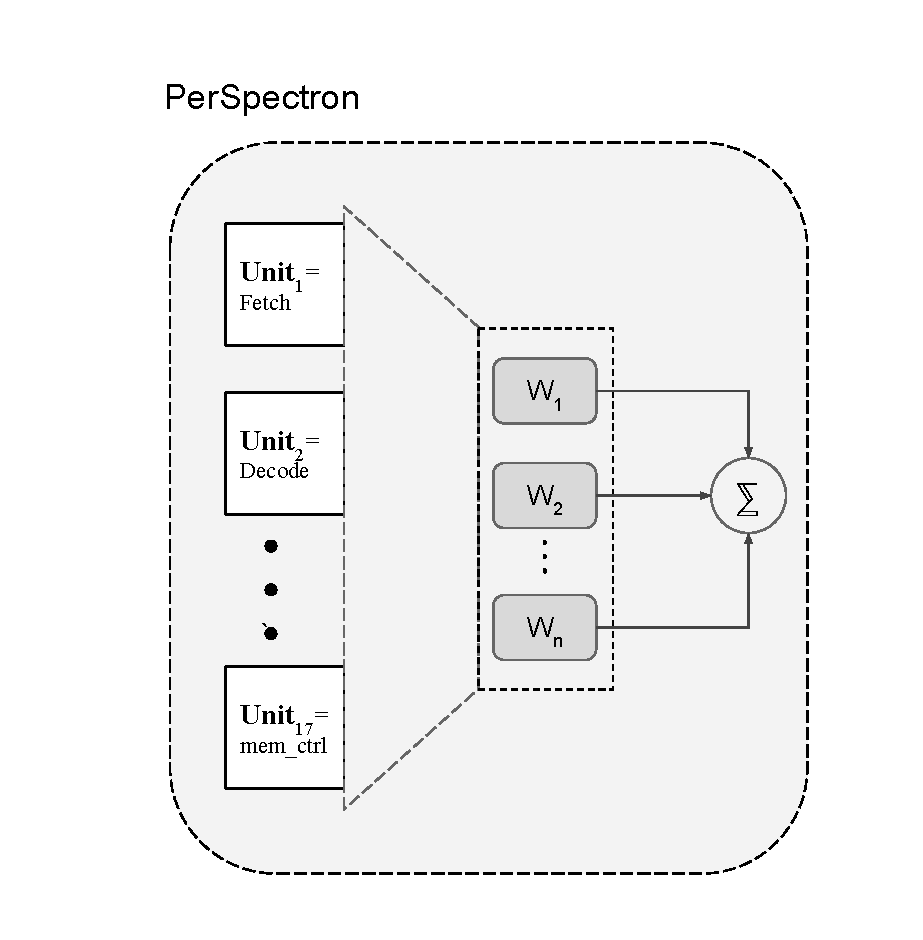
\includegraphics[width=0.45\textwidth, height=0.26\textheight]{PerSpectron-Micro2020-camera-R/img/perSpectron.pdf}
% \vspace*{-4mm}
% \caption{ 
% }
% \label{fig:perspectron}
% \end{figure}

In this work we laverage PerSpectron which is a  hardware detector for microarchitectural attacks which uses a simple one layer neural network,  allowing the use of a simpler architecture, which could efficiently 
handle more complex footprints of attacks. 
PerSpectron also included the mutually correlated features from all the components of processors in the feature set. They showed that it is essential for detecting unseen variations of attacks as the information about attacks moves around the processor.


PerSpectron~\cite{PerSpectron} algorithm extracted 106 microarchitectural features that when included in training, it could map a non-linearly separable problem to linear, which was then 
separable by {\em perceptron} and is readily implementable in hardware. An example of such feature is the effect of misses and stalls 
in the Fetch stage. The squashed cycles in each stage, all the ROB, IQ, and 
Register full events, undone maps in the Rename stage, and memory order 
violation in the IEW stage propagate back to the Fetch stage. The relationship 
between these events' Fetch is not a simple cumulative function in an out-of-order 
processor. 
However, features such as \textit{fetch.MiscStallCycle} capture the 
relationship.
The result was competitive 
with a more complex deepNN that is not easily implementable in hardware. Thus, 

\begin{note}

A Perceptron using invariant microarchitectural features of the pipeline can be set up to play an adversarial game with a much more complex deepNN. 

% 
\end{note}
 
In the next section, we explain \scheme and propose an asymmetric GAN training Perceptron automatically for adversarial examples of microarchitectural attacks. We then explain how to control the type of adversarial microarchitectural attack sample generated, followed by a method using the knowledge from the correlations between pipeline features to adaptively train the Perceptron for adversarial examples and reduces the transferability of the Perceptron's parameters. 

\begin{figure*}[ht!]
\centering
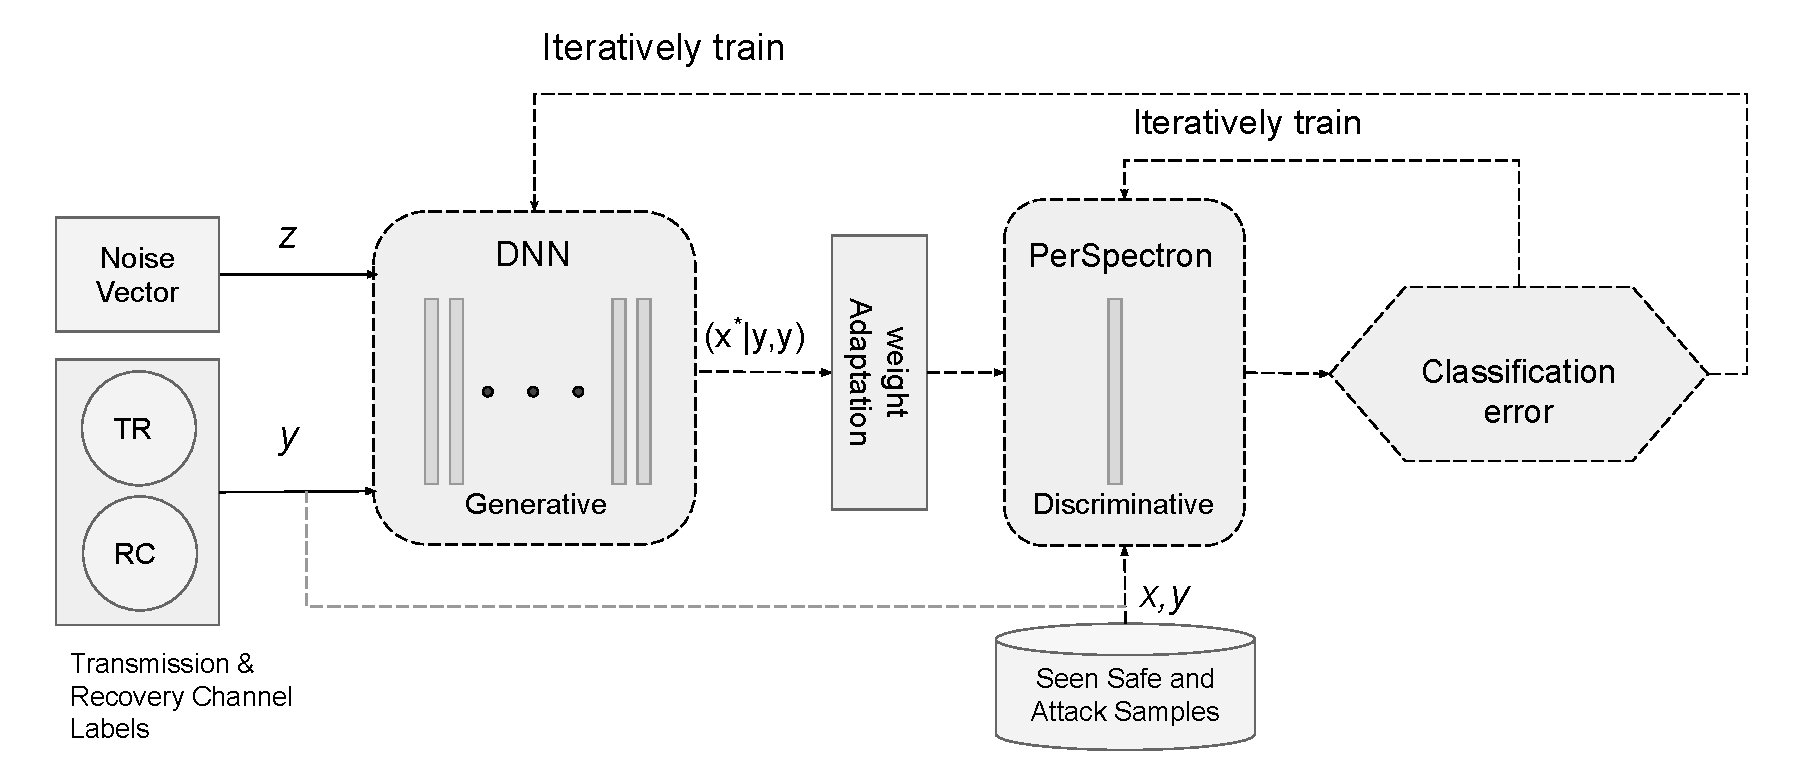
\includegraphics[width=\textwidth]{PerSpectron-Micro2020-camera-R/img/Brutus.pdf}

\caption{\scheme{} Architecture Diagram }

\label{fig:algdiagram}
\end{figure*}

\subsection{{\scheme} Architecture}

{\scheme} uses a deep neural network (DNN) as generator and PerSpectron,  as the discriminator. This differs with original  GANs~\cite{goodfellow2014generative} which uses same convolutional neural
networks (CNNs) in both the discriminator and the generator
architecture of GAN.  The DNN and PerSpectron play an
adversarial game. We introduce this architecture as an {\em asymmetric} GAN, in which a one layer neural network with large number of detailed microarchitectural features, tries to determine whether a particular example is coming from the training dataset or created by the DNN. 

The DNN learns through the feedback it receives from the PerSpectron's classification. 
 Accordingly, each time the PerSpectron is fooled into classifying a generated sample, the DNN knows it did something well. Instead of recognising the pattern, the DNN learns to create them essentially from scratch; indeed, the input into the DNN is mainly a vector of random numbers and labels which we describe in next section.  Conversely each time the PerSpectron  rejects an adversarial attack, the DNN receives the feedback that it needs to improve.

The PerSpectron continues to improve as well. Like any classifier, it learns from how far its predictions are from the true class. 
So, as the DNN generator gets better at producing realistic adversarial samples, the PerSpectron gets better at telling generated samples from original data, and both models continue to improve simultaneously. 


%The equation of loss function is given by [min max equation]. 




% The Generator learns through the feedback it receives from
% the discriminator’s classification. The discriminator’s goal is
% to determine whether a particular example is coming from the
% training dataset or created by the Generator. Accordingly, each
% time the discriminator is fooled into classifying a generated
% sample, the generator knows it did something well. Conversely
% each time the discriminator rejects an adversarial attack, the
% generator receives the feedback that it needs to improve. The
% discriminator continues to improve as well. Like any classifier,
% it learns from how far its predictions are from the true class. So,
% as the generator gets better at producing realistic adversarial
% sample, the discriminator gets better at telling adversarial
% samples from original data, and both models continue to
% improve simultaneously.
%A conditional GAN allows us to direct the generator to synthesize the adversarial example we want.

 




% \subsection{Data Transmit And Recovery Channel Control}
\subsection{Adversarial Attack Type Control}~\label{TypeControl}
 Our DNN generator learns to produce realistic microarchitectural footprint examples for each label in the training dataset and the PerSpectron learns to distinguish generated sample-label pair from real label-sample pairs.   
 In contrast to a design where the Disriminator learns to assign a correct label to each real example in addition to distinguishing real example from fake, our PerSpectron discriminator does not learn to identify which class is which.  It learns to accept matching pair from seen database while rejecting pairs that are mistmatched and pairs in which there are generated by DNN. 
 
 The DNN uses the noise vector and label to synthesize an adversarial example given that or conditioned on the value of the label. The goal of this fake example is to look in the eyes of Discriminator as close as possible to a seen {\em i.e., attack} example for the given label.  
 Accordingly in order to fool the PerSpectron it is not enough for our DNN generator to produce realistic looking footprints of attacks and safe programs. The sample it generates also need to match their labels. After our DNN generator is fully trained, this then allows us to specify what attack type we want to synthesize by passing it the desired label. 
 
 The PerSpectron receives seen samples from dataset  with labels, and generated examples from DNN with the label used to generate them.  PerSpectron learns two things: 
 On the seen data-label pairs it learn
 how to recognize the seen attack and safe data from the generated ones and, second, how to recognize matching pairs generated by the DNN. On the generator-based examples, PerSpectron learns to recognize generated program-labeled pairs, thereby learning to tell them apart from the seen ones. The PerSpectron outputs a single probability indicating its conviction that input is a seen attack, matching pair. 
 
\begin{note}
{In contrary to the original PerSpectron paper, the PerSpectron's goal here is to learn to reject all generated examples and all examples that fail to match their label, while accepting all seen example-label pairs of microarchitectural attacks.}
 \end{note}
 
 Note that for each generated example the same label is passed to both the DNN and the PerSpectron. Also note that the DNN is never explicitly trained to reject mismatched pairs by being trained on the seen examples with mismatching labels; its ability to identify mismatched pairs is a by-product of being trained to accept only seen matching pairs. 
 
 
\noindent\textbf{Train the DNN}:
For each training iteration:

%\begin{compactitem}
\begin{itemize}  [topsep=0pt,parsep=0pt,partopsep=0pt, label={--}, leftmargin=*] %[leftmargin=*] noitemsep
\item  The DNN takes a new random noise z and three labels: A the transmission channel type of the attack {\em i.e., meltdown-type}, A the recovery channel type of the attack {\em i.e., prime+probe-type} and the class target $t$ {\em i.e., safe or suspicious}. DNN generates an example $x^{\star}$ that strives to be both an adversarial attack (or a realistic safe program) and a convincing match for the labels $TC$ and $RC$.  

\item PerSpectron network classifies $x^{\star}$ into 0/1. One for matched seen sample-labels from the dataset and 0 for unmatched sample-labels and generated sample-labels.    

% \item Compute the classification error and backpropogate the total error to update PerSpectron's  weights, seeking to minimize it's classification error. 

\item  The classification error of PerSpectron will be computed and backpropogated to update the DNN weights, seeking to maximize the PerSpectron's error. 

\end{itemize}

%\end{compactitem}

\noindent\textbf{Train the PerSpectron:}
For each iteration:

%\begin{compactitem}
\begin{itemize} [topsep=0pt,parsep=0pt,partopsep=0pt, label={--}, leftmargin=*]
%[labelindent=0pt]%[leftmargin=*] noitemsep
\item We choose a seen program sample $x$ from the training dataset with its two labels: the transmission channel type $TC$ of the attack {\em i.e., meltdown-type}, A the recovery channel type $RC$ of the attack {\em i.e., prime+probe-type} 
% the class target $t$ {\em i.e., safe or suspicious}. 
 
\item DNN gets a new random noise vector $z$ and label $TC$ and $RC$ and  synthesize an adversarial example  $x^{\star}$.
 
\item PerSpectron receives the seen sample example $x$ with label $TC$ and $RC$ and  the adversarial generated sample-label $x^{\star}$ and the labels that were used to generate them $TC$ and $RC$. For both examples PerSpectron outputs a probability  indicating whether the input example was a seen data from dataset, matching its label pair and  for a generated data or unmatched pairs (0/1). 
 
\item The classification error of PerSpectron will be computed and backpropogated  to update it's weights, seeking to minimize it's classification error. 
 
\end{itemize}
%\end{compactitem}

% 
The training ends when our GANs reaching Nash equilibrium. Which happens when the following conditions are met: DNN produces fake examples that are not distinguishable from the seen attacks in the training dataset. The PerSpectron can at best randomly  randomly guess whether a particular example is a seen attack or a generated adversarial one. All examples produced by our DNN at this points with feeding various categories of attacks to it, are adversarial attack samples which carry the footprints of microarchitectural attacks but are very hard to distinguish. 


In the next section we explain how to use the generated adversarial samples to train the original PerSpectron classifier. 

\subsection{Training on Adversarial Examples}

We want to use GANs to create a large dataset, but we need a large dataset to train the GAN in the first place. GANs are notoriously hard to  train. As with any other cutting-edge field, opinions about what is the best approach are evolving specially no study has been done on microarchitectural data.
On the other hand, attack programs include safe code segments. This is like feeding a GAN a partial frame of an image which is common between different faces. Eventually GANs learn to identify the exact footprints of certain class and will generate adversarial based on those but the safe code segments of attack programs slows down the training of GANs leading to further need for more samples, a catch 22 situation. We solve this problem through the following:


First, we use standard data augmentation using program synthesising to create a larger dataset of all the attack, this samples does not add to the diversity of examples as we discussed in section~\ref{intro} and ~\ref{results} but it helps our GAN to converge faster. 

Second, instead of training our GAN on the whole attack program, we train on samples taken from attacks atomic tasks only.  ”Atomic
Tasks” are operations that, if interrupted, will disable the attack: For example, Flushing cache lines, mistraining branch predictor  or
Attempting to infer the secret byte that is loaded into cache.
This enables the GAN to automatically generate adversarial examples of tasks related to the attacks regardless of the safe code segments presented in those attacks.

Third, we use this dataset to train a GAN to create adversarial attack sample-pairs as we explained in section~\ref{TypeControl}. We input two labels to our DNN, the transmission type of the attack {\em i.e., meltdown-type } and the recover type of the attack {\em i.e., prime+probe-type}. The generator will generate label-conditioned adversarial attacks that misleads the PerSpectron classifier. 
Finally, we use the augmented dataset from step 1 along with the GAN-produced adversarial samples from step 2 to train the PerSpectron. 

 

  

 
\subsection{Adaptive Adversarial Learning}

Prior works showed that microarchitectural features are mutually correlated in different components of processors~\cite{PerSpectron}. This is due to the nature of components of pipeline, and their interleaved functionality in an out of order superscaler processor. For example, \textit{IcacheSquashes}, \textit{MiscStallCycles} and \textit{PendingTrapStallCycles} 
are mutually decorrelated in the fetch unit but they have high correlation with stalls 
and traps in other components, {\em i.e.} \textit{commit.NonSpecStalls}, 
\textit{lsq.thread0.rescheduledLoads} and \textit{dcache.blocked:no\_mshrs}. This property has been used in prior work~\cite{PerSpectron} to produce {\em replicated detectors} to improve the detection as the attack footprint moves in the pipeline.



To improve the security and robustness of forensic detectors and
standard ML-based to mitigate the adversarial machine learning attacks, 
many considered random feature selection
strategy
~\cite{nowroozi2020survey, secureDetection2019}.
 In this work instead of random selection of features or  dynamically switching between different classifier, we leverage  mutually correlated microarchitectural features from the replicated detectors in different components of processor to reduce the transferability of classification parameters, and increase the security of our 
detection. 

% We apply adaptive feature weight elimination during adversarial training, in country to previous works whichr. 
Our adaptation is embedded in Perceptrons weight from the training phase.  Our adaptive training is very simple. We first group the microarchitectural features into mutually correlated sets {\em e.i.,} one feature per component of pipeline. During training we add a layer between our DNN and PerSpectron. This layer chooses one feature from each mutual group and sets the corresponding weight output values from the  generator to zero.

Incredibly, this simple addition drastically improves accuracy on adversarial attacks, by ensuring that network doesn't become overdependant on certain units or groups of features that in effect just remember observation from training set. With weight adaptation perceptron can not rely too much on any one units or features of the processor. Therefore, perceptron weight updates are more evenly distributed throughout the adversarial training. This makes perceptron learning much better at generalizing to unseen attacks. 

\begin{note}
\scheme{} has been trained with weight clipping to produce accurate predictions on adversarial examples even under unfamiliar conditions, such as those caused by dropping a highly correlated feature.
\end{note}
 At test time the weight adaptation layer doesn't remove any weight so that the full Perceptron is used for prediction. 



\subsection{\scheme{} Equilibrium State }
In original GAN, because the two agents only competing against each other, it makes sense that the Generator's loss would be a negative of the discriminator. In our case a perceptron discriminator is competing against a DNN as the generator.  So far we are never given a clear set of conditions under which the training has finished in practice.
We use a stopping criteria that significantly improve on the loss function, which are now interpret-able and provide clearer stopping criteria. We try to minimize the distance between the expectation of the real attack and the expectation of the generated distribution.  

% \begin{figure}[ht!] 
% \centering
% 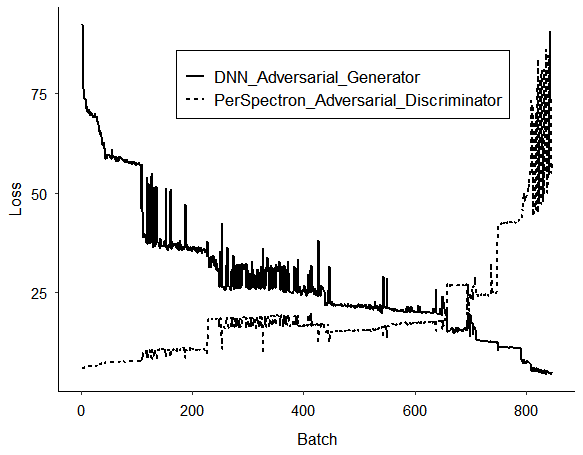
\includegraphics[width=0.49\textwidth]{PerSpectron-Micro2020-camera-R/img/Loss.png}
% \vspace*{-4mm}
% \caption{The generators loss decreases after several training iterations.  
%  % \scheme{} 
%  }
% \label{fig:sature}
% \end{figure}

Figure~\ref{fig:sature} shows the loss value of our DNN adversarial example generator and PerSpectron-based Adversarial Discriminator. The y-axis is the loss function for the DNN and the PerSpectron outcome for the likelihood of the generated example, whereas the horizontal axis shows the adversarial training batch. After suitable number of epochs, the discriminator will have found an equilibrium that allows the generator to learn meaningful information from the discriminator. 


\begin{figure}[ht!] 
\centering
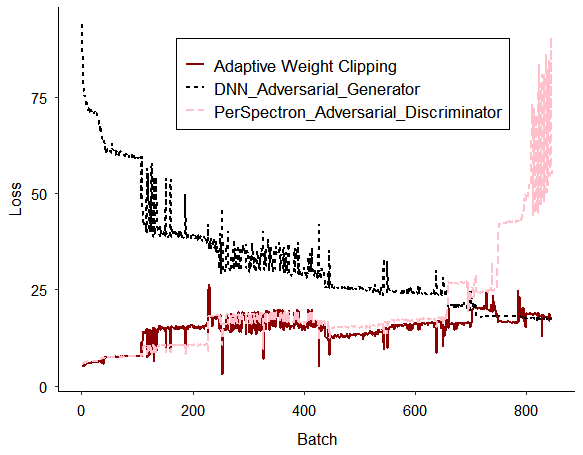
\includegraphics[width=0.49\textwidth]{PerSpectron-Micro2020-camera-R/img/Loss2.png}
\vspace*{-4mm}
\caption{The generators loss decreases after several training iterations. After suitable number of epochs, the PerSpectron finds an equilibrium that allows the DNN generator to learn meaningful information from the discriminator. Weight clipping during adversarial training prevents the generator to find a single observation of adversarial attack examples that always fool the PerSpectron.  }
 
\label{fig:sature}
\end{figure}






